\chapter{Migration process}

This chapter describes the process of migrating a web application to serverless architecture. The goal of the migration is to explore the feasibility of the catalogued patterns by applying them on common problems in the domain of web application development. In cases where the patterns prove insufficient or unsuitable to the problem in hand, modifications or new patterns are proposed. As well as exploring the patterns we're seeing how the distinct serverless features drive application design and trying to gain deeper understanding of the advantages and shortcomings of the paradigm. Finally in chapter \ref{cha:evaluation} the migration outcome is evaluated against the pre-migration application in terms of quality and ease of development.

\section{Image Manager}

The migrated application, Image Manager, is a tool for managing image assets. The application is adapted from a real-world work assignment, although modified in places for the sake of illustration. Similarly to a SaaS offering such as Cloudinary, the application takes user-uploaded images, performs various forms of processing and then hosts and serves the processed images to be consumed by other applications. In case of Image Manager the processing needs are threefold: rendering a thumbnail, rendering a low quality image placeholder (LQIP), and automatic label detection. Thus in short, Image Manager can be split into three basic functional requirements: image upload, image processing and image hosting.

The pre-migration serverful Image Manager consists of a single server application that connects to a number of cloud services. These components are depicted in figure \ref{fig:serverfulArchitecture}. The server application publishes a single HTTP API endpoint for image uploads which is consumed by a browser client. In place of access control this public-facing API uses a CAPTCHA: before image upload the client requests a challenge from Google reCAPTCHA API, solves it and sends the obtained token along with the image upload request. The server application then also connects to reCAPTCHA API to verify token validity before proceeding with the upload request. A CAPTCHA is used instead of full-blown authentication to allow for anonymous users while still providing some degree of protection against bots and other illicit usage. After CAPTCHA verification the application proceeds with image processing. The thumbnail and LQIP rendering tasks are performed locally whereas labeling is handled by a network call to an external image analysis service, Google Cloud Vision API. The three processing tasks are independent and performed concurrently. Finally both the original and processed images are uploaded to Google Cloud Storage where they can be fetched via publicly accessible URLs. Figure \ref{fig:serverfulSequence} illustrates the image upload sequence in further detail, showing how the components fit together.

\begin{figure}[h]
  \centering
  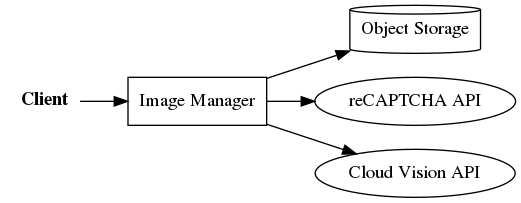
\includegraphics[width=0.65\textwidth]{image-manager.png}
  \caption{Serverful Image Manager components}
  \label{fig:serverfulArchitecture}
\end{figure}

\begin{figure}[h]
  \centering
  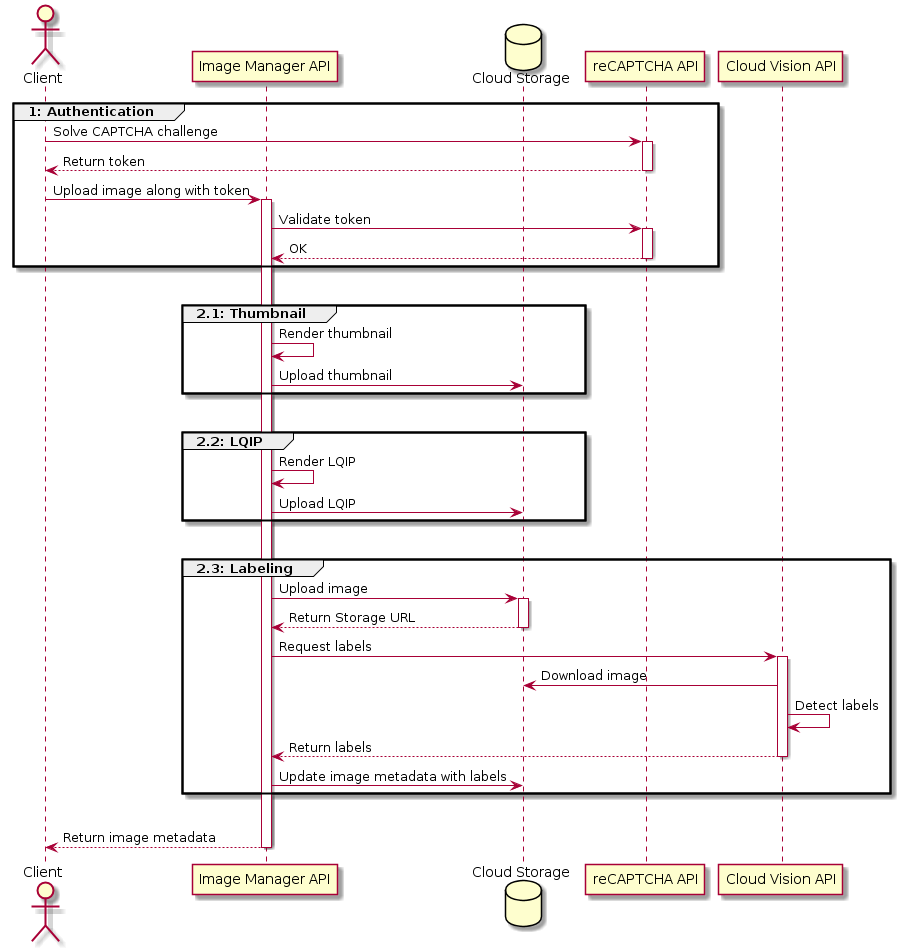
\includegraphics[width=0.90\textwidth]{sequence.png}
  \caption{Serverful Image Manager upload sequence}
  \label{fig:serverfulSequence}
\end{figure}

Overall the image upload task is both CPU-intensive due to local rendering and IO-heavy due to cloud service requests and also since processing results are temporarily written on disk before cloud storage upload. Image Manager is written in TypeScript, transpiled into JavaScript and running on NodeJS v10. The server application is containerized into a Docker image and deployed on a single VM on Google Cloud Platform's \textit{us-east1} region. The VM exposes an IP address through which the application is accessed from public internet.

The motivation to migrate Image Manager to serverless architecture arises from four main shortcomings in the current implementation: availability, scalability, cost-efficiency and isolation. First, the obvious drawback of the server application's single-VM deployment is poor availability as there is no failover instance to take over in case of VM failure. Likewise the application's capacity to serve traffic is limited by a single VM's computing resources as there is no scaling mechanism in play. Achieving this double goal of availability and scalability, i.e. ensuring a correct number of VMs to meet current demand at all times would require a considerable amount of infrastructure configuration involving load balancing, clusterization and scaling policies (TODO source?). This inelasticity also results in cost-inefficiency as the VM instance is constantly running and accumulating charges whether or not there's any traffic. Notably the cloud services connected to by the server application do not contribute to this cost-inefficiency as they follow a pay-per-use pricing model. Finally the current implementation suffers from a lack of isolation, primarily since all application logic including image processing tasks are bundled together into a single application. This causes resource contention, as for example high CPU usage in one of the rendering tasks can divert resources from the API and result in connection timeouts. This combined with processing tasks' highly asymmetrical performance profiles also further complicates scaling as we can only scale the whole application, not parts of it. Lack of isolation also presents itself in how all traffic is routed through the server application, which in case of image uploads means an extra network trip before reaching Cloud Storage.

\section{Serverless implementation}

keep using same services, only server application changes. used in different ways too

Pattern selection:
client is a Thick Client
authentication uses Valet Key
processing triggered as Event Processor, branches off to Fan-out/Fan-in
processing tasks isolated, Bulkhead, can scale independently
for which need was pattern X chosen?

\ref{fig:serverlessArchitecture} presents the migrated serverless architecture, where the same functionality is split into separate serverless functions and tied together in an event-driven flow. In both figures rectangular boxes represent the parts that are implemented by hand, whereas the rest are external services. \ref{fig:serverlessSequence} illustrates the image upload sequence in our serverless implementation.

% TODO Building both deployment artifacts from the same code base. describe migration process step-by-step? API, authentication, processing and upload?

\begin{figure}[h]
  \centering
  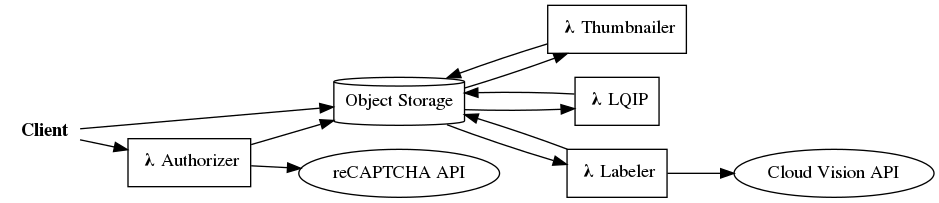
\includegraphics[width=\textwidth]{image-manager-serverless.png}
  \caption{Serverless Image Manager architecture}
  \label{fig:serverlessArchitecture}
\end{figure}

\begin{figure}[h]
  \centering
  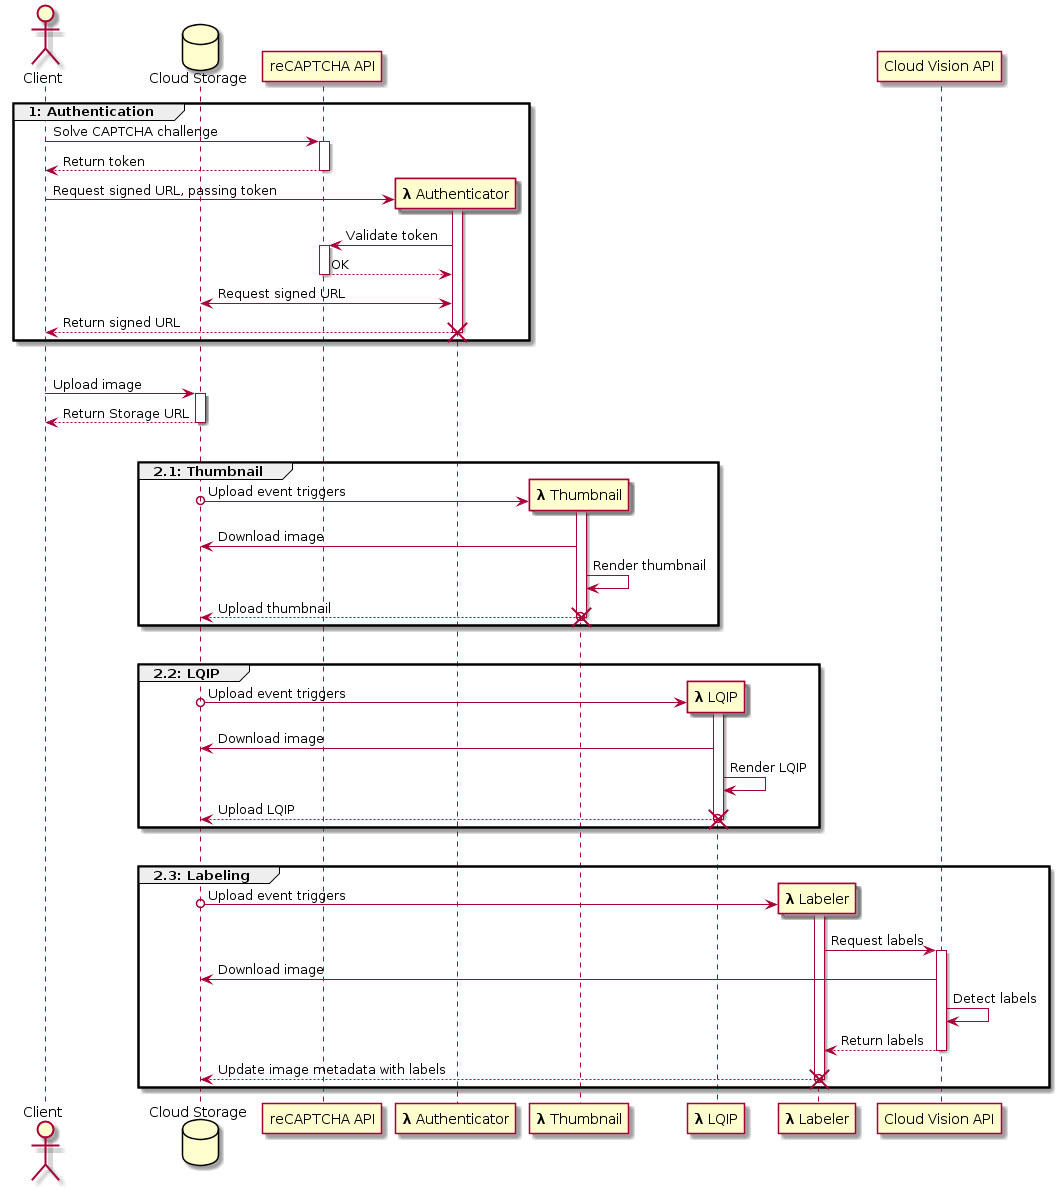
\includegraphics[width=0.90\textwidth]{sequence-serverless.png}
  \caption{Serverless Image Manager upload sequence}
  \label{fig:serverlessSequence}
\end{figure}

\section{New patterns} \label{sec:newPatterns}

Here are some patterns to address problems I came across while sketching out the above serverless implementation:

\subsection{Fetcher} \label{subsec:Fetcher}
% or Local Threader?

\textbf{Problem:} Scaling an IO-bound operation out to parallel function instances is inefficient since the instances compete of the same IO resources.

\textbf{Solution:} Use local threading inside a single function instance to efficiently scale out operations like network requests.

E.g. three parallel functions each making a network request, or three parallel functions invoked by cloud storage upload that start execution by downloading the image: is it more efficient to have one function download the image and then invoke/pass the image as argument to three processing functions?

\subsection{Asynchronous Response} \label{subsec:AsyncResponse}

\textbf{Problem:} The client doesn't get any feedback from the asynchronous tasks it triggers.

\textbf{Solution:} Use a pub/sub channel to send a message to the client at the end of the task.

\subsection{Task Manager} \label{subsec:taskManager}

\textbf{Problem:} The client, after triggering an asynchronous task, has no way of tracking task progress or cancelling it.

\textbf{Solution:} Make each function instance subscribe to a pub/sub channel in the beginning of its execution in order to listen to client commands.

The former is one-way pub/sub, in Task Manager the function also subscribes.

\subsection{Throttled Recursion} \label{subsec:throttledRecursion}

\textbf{Problem:} Recursive serverless functions can overwhelm downstream resources by scaling out quickly or result in an infinite loop.

\textbf{Solution:} Pass recursive invocations through a message queue in order to control recursion speed.
